\begin{itemize}
\item Static analysis technique to detect dependencies.
\item We use these dependencies to generate data structure for scheduling interrupted rules.
	\begin{itemize}
	\item Each entity maintains a list of entities depending on it, and a list of inactive rules.
	\item Maintaining the list according to the dynamics of entities in the game (creation, update, and removal).
	\end{itemize}
\item To what extent a game can benefit from such an optimization? Game state changing too fast. Optimization data structures create overhead which surpass the performance gained by our scheduling.
\item Dynamic analysis technique to detect the update frequency.
\item Rules that update too often will not benefit from our optimization and are not included.
\item The choice of the update threshold depends on the data structure we are using for the optimization.
\item Further optimization: data structures can be stored in the world instead of locally into entities for better cache coherence.
\end{itemize}

A problem that arises from the use of some of these operators is that of \textit{busy waiting}. For instance, the healer behaviour requires that he waits for a guard to ask for healing before leaving the guard post. To describe this behaviour we must continuously check if a wounded guard is nearby. The overhead of this operation is minimum for just one guard, but for a greater amount of guards this can seriously affect the game performance, since it is required that the healer checks if any guard is close enough at every game frame. This observation can be generalized for rules which wait for a condition on values of the game state altered by other rules. Consider the following example in Casanova 2:

\begin{lstlisting}[mathescape]
entity E = {
   A : int
	
   rule A = //rule $r_{1}$
      wait 1.0
      yield A + 1
   rule A = //rule $r_{2}$
      wait A % 2 = 0
      //execute rule body $b_{2}$
   rule A = //rule $r_{3}$
      wait A % 5 = 0
      //execute rule body $b_{3}$
   rule A = //rule $r_{4}$
      wait A % 10 = 0
      //execute rule body $b_{4}$
      
   Create() = {A = 0}		
}
\end{lstlisting}
In the snippet of code shown above, rule $r_{1}$ increments the field A by 1 every second. Rules $r_{2}$, $r_{3}$, and $r_{4}$ wait until A is multiple of respectively 2, 5, and 10 before executing the rest of their bodies. If we assume that running rule bodies $b_{2}$, $b_{3}$, and $b_{4}$ take 0.5 seconds, and we consider a time span of 12 seconds, then $r_{2}$ will be inactive for 10 seconds and run for 2 seconds, $r_{3}$ will be inactive for 11 seconds and run for 1 seconds, and $r_{4}$ will be inactive for 11.5 seconds and active for 0.5 seconds. This comparison is shown in Figure \ref{fig:s4f1}. The time amount in the light grey bars is spent by rules by busy waiting, since in that time interval they keep checking the synchronization condition. We observe that the reactivation of a rule body execution depends only on a change on the fields used in the boolean expression of the \texttt{wait} operator, and this change can only be performed by other active rules (in our example only $r_{1}$, but in a more general case there could be more than one rule acting on the same field). From this consideration we argue that we can make waiting dependent on the game state rather than on the rule state.

\begin{figure}
	\centering
	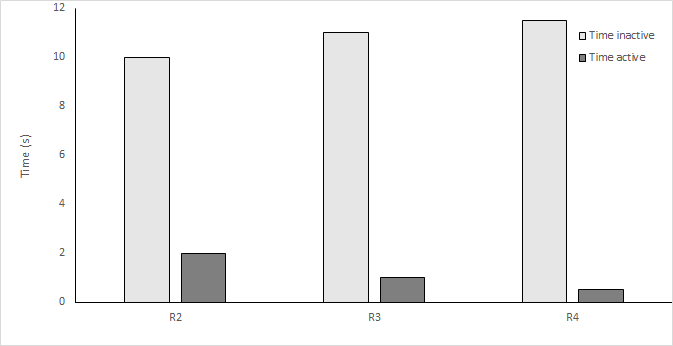
\includegraphics[scale=0.5]{Image/wait_chart}
	\caption{Chart showing the time spent by inactive and active rules}
	\label{fig:s4f1}
\end{figure}

Given that the evaluation of a waiting condition changes only when at least one of the fields affecting it has changed, we keep track of all rules waiting for a change on that field (this can be done statically by examining the expression of a \texttt{wait} operator). When a rule evaluates the condition of a \texttt{wait} operator, if the condition evaluates to \texttt{false}, it is suspended. When another rule changes a field, it resumes any suspended rules with that field. Suspended rules evaluate again the \texttt{wait} conditions. Those which evaluate to \texttt{false} remain suspended, those which evaluate to \texttt{true} become active again and proceed with their execution.

The other operators affected by busy waiting are the concurrency operator and the pre-emption operator (the parallel operator keeps executing its code continuously and it does not wait for any condition itself, although its body can contain other operators that do).